\documentclass{article}
\PassOptionsToPackage{numbers,sort&compress}{natbib}
\usepackage[dblblindworkshop]{../shared/neurips_2026}
\workshoptitle{RoboPAD: Post-Training Adaptation of Robot Foundation Models}
\usepackage[T1]{fontenc}
\usepackage[utf8]{inputenc}
\usepackage{microtype}
\usepackage{booktabs}
\usepackage{array}
\usepackage{graphicx}
\usepackage{amsmath,amssymb}
\usepackage{enumitem}
\usepackage{siunitx}
\sisetup{group-digits=false, table-number-alignment=center, retain-explicit-plus=true}
\usepackage[hidelinks]{hyperref}
\usepackage{placeins}
\title{Refinement versus Refresh:\\
Compute Allocation for Closed-Loop Robot Policies}
\author{Anonymous Authors}
\begin{document}
\maketitle

\begin{abstract}
How should a chunked robot policy spend inference compute: refine its current
action chunk, or replan from a newer observation? We introduce a reproducible
protocol for evaluating this trade-off within a frozen policy and use one frozen
SmolVLA checkpoint as a worked case study. The protocol
defines refinement and refresh separately, measures complete generation and
episode expenditure, separates discovery from held-out evaluation, freezes
confirmatory comparisons before outcomes are observed, and labels later analyses
as descriptive. The case study runs in synchronous LIBERO simulation.
The denoising comparisons were frozen before confirmation; refresh-prefix
contrasts were added later and are interpreted descriptively. In the
prespecified primary comparison, at a fixed two-action prefix, reducing
denoising from five to two steps increased success from 122/160 to 139/160 while
reducing counted arithmetic. Full-generation calibration showed that 82.1\% of
native arithmetic was independent of denoising. An amended descriptive comparison
observed 138/160 versus 139/160 successes when refreshing after five rather than
two actions, with 60.7\% lower arithmetic per attempt; equivalence was not
established. A simple cost-aware rule matched the fitted model's choices.
These checkpoint-specific findings illustrate the protocol; they do not define
a general SmolVLA or cross-policy allocation rule. The transferable contribution
is the procedure for evaluating success, compute, and evidence status together.
\end{abstract}

\section{Introduction}

A robot policy can reduce inference work in two ways: spend less computation
refining each action prediction, or execute more actions before requesting a
new prediction. These interventions affect behavior differently. Reduced
refinement changes the prediction itself; longer execution prefixes delay
observation-conditioned revision and expose later positions of the predicted
action sequence. Their relative value should therefore be evaluated through
closed-loop outcomes under a common resource constraint.

We ask: \emph{given a fixed inference budget, how should a robot divide
computation between prediction refinement and observation-conditioned refresh?}
The cost of a fresh prediction makes this question nontrivial. In the frozen
SmolVLA case study \cite{smolvla}, work independent of denoising accounts for
82.1\% of native counted arithmetic. For this checkpoint, reducing refinement
therefore leaves a substantial cost per generation: sufficiently tight budgets
require less frequent refresh even at low denoising counts. This cost boundary
determines what is feasible, but not which feasible setting controls the robot
best.

We operationalize this allocation question through two within-checkpoint
comparisons. The primary comparison varies denoising at a fixed execution prefix
to evaluate whether additional refinement improves success. A complementary,
descriptive comparison varies the execution prefix at fixed denoising to examine
whether more frequent refresh justifies its additional expenditure. We evaluate
twelve configurations in a paired 480-attempt discovery study, then seven
configurations in 1,120 confirmation attempts on eight tasks excluded from
selection. Three frozen comparisons evaluate refinement. The amended
prefix comparisons examine refresh; they neither isolate observation freshness
from action-position effects nor establish an optimal allocation rule.

Within the SmolVLA case study, the primary two-action prefix with two denoising
steps yields 139/160 successes versus 122/160 for five steps, with lower reference
arithmetic. At two denoising
steps, however, a five-action prefix yields 138/160 successes at 60.7\% less
arithmetic per attempt than the two-action prefix; their quality difference
remains unresolved. A simple cost-aware rule also matches the fitted response
model's choices at all three ceilings, with no demonstrated selection advantage
from fitting.

These checkpoint-specific outcomes demonstrate how to apply the protocol and
how its evidence boundaries constrain the resulting claims.

The contributions are:
\begin{itemize}[leftmargin=*,nosep]
    \item a reproducible refinement--refresh protocol that defines the controls,
    accounts for complete prediction and episode expenditure, and freezes
    confirmatory comparisons before held-out evaluation;
    \item an evidence-reporting procedure that keeps prespecified refinement
    tests separate from amended descriptive refresh contrasts and retains their
    uncertainty and provenance; and
    \item a paired SmolVLA study that demonstrates the protocol across twelve
    discovery configurations and seven held-out confirmation settings.
\end{itemize}

\section{Related Work}

Resource-allocation studies motivate evaluating configurations across explicit
budgets. Chinchilla studies model-size and training-data allocation
\cite{chinchilla}; embodied scaling studies consider world modeling, behavior
cloning, and closed-loop forecasting and planning
\cite{pearcescaling,motionscaling}. Our comparison instead varies deployment
refinement and execution prefix within a fixed policy. Work distinguishing
FLOP-optimal from elapsed- or monetary-cost-optimal allocation
\cite{beyondchinchilla} also motivates retaining separate resource coordinates.

VLA-Perf characterizes inference performance across denoising, chunk size,
asynchronous execution, and hardware/runtime choices \cite{vlaperf}.
SmolVLA studies asynchronous inference and robot behavior \cite{smolvla}.
Here predicted chunk size remains fixed, while executed prefix changes; task
success is measured alongside computation. RoboMonkey studies test-time sampling
and action verification \cite{robomonkey}, an adjacent allocation axis that
would require counting candidate generation and verification costs.

Adaptive VLA scheduling is directly related. DVAC uses denoising-derived action
variance to choose an execution prefix before replanning \cite{dvac}.
ElegantVLA schedules vision--language recomputation or reuse together with action
denoising modes \cite{elegantvla}. Our study instead compares fixed configurations
under explicit arithmetic ceilings and freezes separate-task denoising
comparisons. It neither introduces an adaptive scheduler nor establishes an
advantage over these methods; their reported speedups have different policies,
hardware, and measurement boundaries.

\section{Protocol for Refinement--Refresh Evaluation}
\label{sec:allocation}

The protocol has four stages. First, define refinement and refresh as separate
deployment controls while holding the checkpoint and paired rollout conditions
fixed. Second, measure complete prediction cost and realized episode expenditure
under an explicit counting boundary. Third, use discovery data to freeze the
confirmatory comparisons before held-out outcomes are observed. Fourth, report
success and expenditure together, label any later contrasts as descriptive, and
avoid interpreting arithmetic savings as latency improvement or similar observed
success as equivalent quality. The following subsections instantiate each stage.

\subsection{Compute rate and episode expenditure}

Let $K$ be the predicted action-chunk length and $h<K$ the execution prefix.
At each policy query, the policy predicts $K$ actions, executes only the first
$h$, discards the remaining $K-h$, and then generates a new chunk from a new
observation. Thus $h$ controls replanning frequency without changing the
predicted chunk length. In all experiments, $K=50$. We reserve $T_e$ for the
number of actions actually executed in attempt $e$. Let $d$ be the denoising
count and $F_{\mathrm{gen}}(d)$ the reference-calibrated neural arithmetic for a full
action-chunk generation at denoising setting $d$. For complete execution prefixes, the nominal
compute rate per simulated control step is
\[
 b(h,d)=\frac{F_{\mathrm{gen}}(d)}{h}.
\]
For a candidate set $\mathcal C$ and budget ceiling $B$, the allocation target is
\begin{equation}
 (h^\star,d^\star)(B)\in
 \arg\max_{(h,d)\in\mathcal C:\,b(h,d)\le B}
 p_{\mathrm{success}}(h,d).
 \label{eq:allocation}
\end{equation}
A configuration need not exhaust the ceiling. This is a deployment compute-rate
constraint for a fixed checkpoint, rather than a training-plus-deployment
objective.

Figure~\ref{fig:closed-loop-policy} summarizes the execution loop. Each policy
call predicts a fixed-length chunk, executes only the first $h$ actions, discards
the remainder, and refreshes from the resulting observation. The denoising
count $d$ controls refinement inside the policy call, while $h$ controls how
frequently the policy receives a new observation.

\begin{figure}[t]
\centering
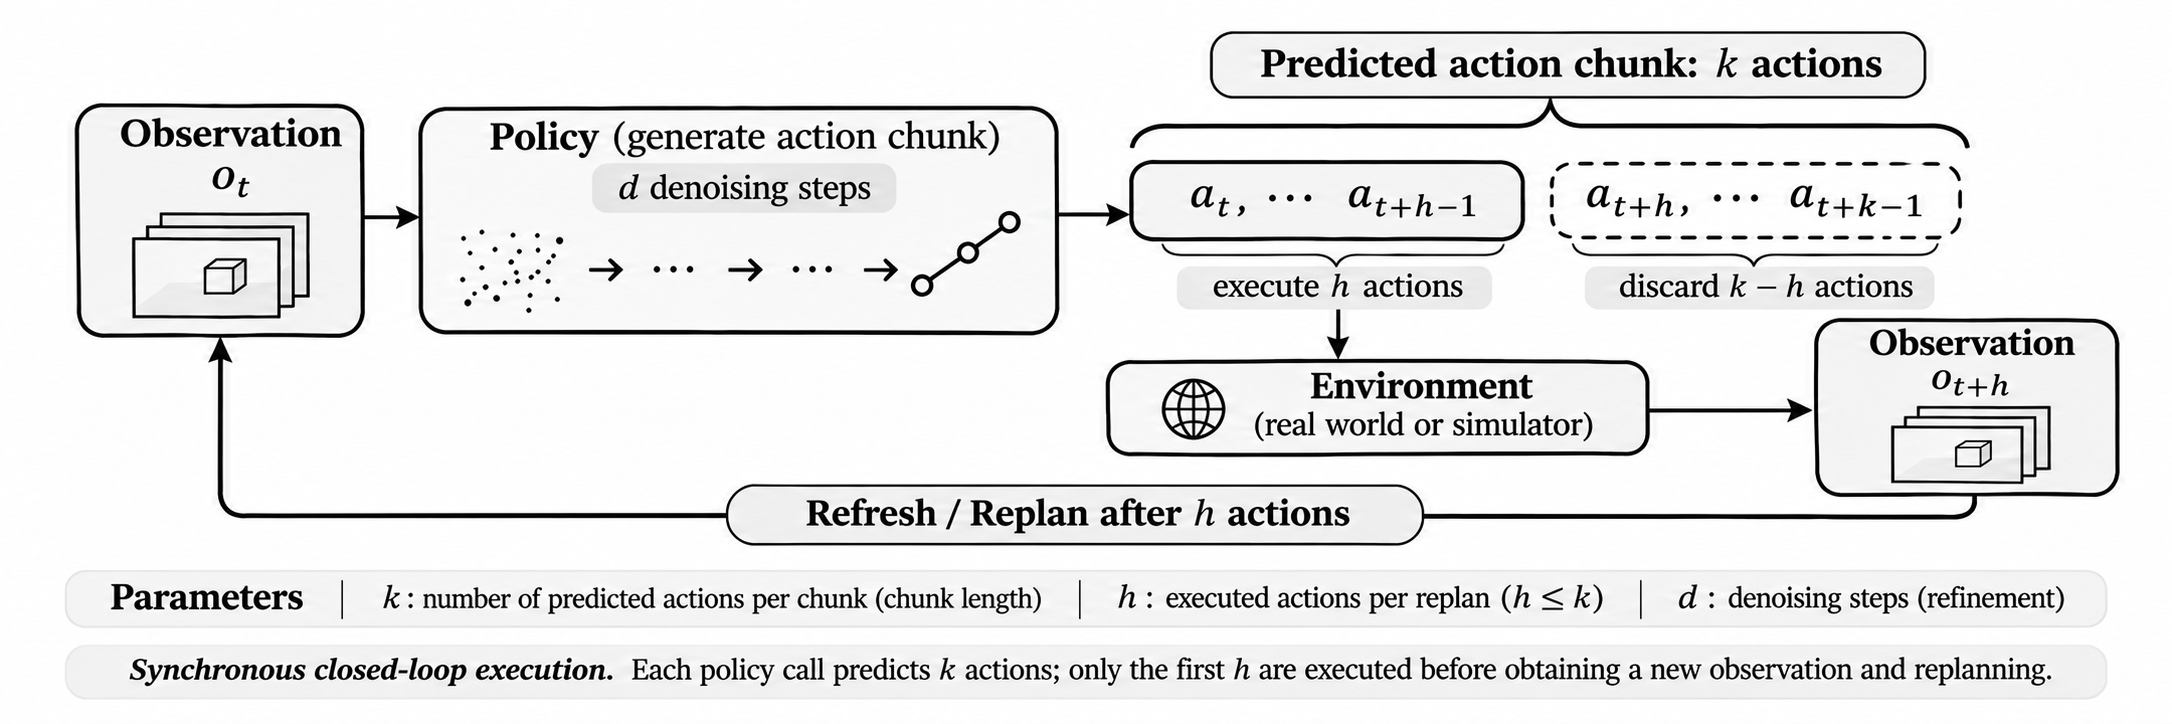
\includegraphics[width=\linewidth]{figures/closed_loop_policy_diagram.png}
\caption{Closed-loop execution used throughout the protocol. Each policy call
predicts $K$ actions after $d$ denoising steps, executes the first $h$, discards
the remainder, and replans from a new observation. In the experiments, $K=50$.}
\label{fig:closed-loop-policy}
\end{figure}

We distinguish this rate from total arithmetic per attempted episode. If attempt
$e$ executes $T_e$ actions, its generated-chunk expenditure is
\begin{equation}
 C_e=\left\lceil T_e/h\right\rceil F_{\mathrm{gen}}(d).
 \label{eq:episode-cost}
\end{equation}
The final generated chunk is charged even if only part of its execution prefix
is used. All-attempt means include unsuccessful episodes. Different trajectories
and termination times can therefore change expenditure at the same nominal rate.
FLOPs, host elapsed time, and CUDA-stream time retain separate units and
measurement boundaries.

\subsection{The fixed cost of a fresh prediction}
\label{sec:results}

Complete-generation profiling counts matrix products, convolutions, and
attention across vision, language prefill, and the action expert, using two
FLOPs per multiply-add. Embedding lookups, normalization, activations,
elementwise arithmetic, and external preprocessing are excluded. We therefore
refer to \emph{dense neural arithmetic}, not an exact count of every scalar
operation. Calibration uses one real development observation and fixed tensor
shapes; its protocol is detailed in Appendix~\ref{app:calibration}.

For the case-study checkpoint and reference input, the measured arithmetic satisfies, to rounding,
\[
 F_{\mathrm{gen}}(d)\simeq 527.108+11.457d\quad\text{GFLOPs}
\]
at all six calibrated denoising settings. Native generation at $d=10$ costs
641.675 GFLOPs, of which 82.1\% is independent of $d$. Halving denoising from
ten to five saves 8.9\% of counted generation work; reducing it to two saves
14.3\%. Equivalently, relative to native deployment $(h,d)=(1,10)$,
\[
 \frac{b(h,d)}{b_{\mathrm{native}}}
 \simeq \frac{0.821+0.179(d/10)}{h}.
\]

We prespecify compute-rate ceilings of $0.25$, $0.50$, and $1.00$ times native.
Eligibility uses measured per-$d$ values, not the rounded affine expression.
For example, $(1,2)$ costs 0.857 times native rate and is ineligible at half-native
budget, whereas $(2,2)$ costs 0.429 times native. The denoising-independent work
alone excludes $h=1$ at half-native budget and $h\leq2$ at quarter-native budget.
A tighter budget can therefore force a longer execution prefix before any
quality-based choice is made. This is an implementation-specific arithmetic
floor under the declared counting boundary, not a universal VLA scaling law.

Calibration uses a fixed input shape; a separate language-length audit leaves
eligibility unchanged under the original absolute ceilings
(Appendix~\ref{app:shape-audit}). Reference arithmetic remains distinct from
task-shaped arithmetic and elapsed time. For the case-study implementation on a fixed input, reducing $d$ from 10
to 5 lowers measured host generation time by 40.5\% while counted arithmetic
falls by 8.9\% (Appendix~\ref{app:fixed-timing}); FLOPs are therefore not a
latency proxy. The cost model defines feasible
schedules; the following experiments ask which feasible expenditures help
closed-loop control.

\section{Applying the Protocol to Frozen SmolVLA}
\label{sec:method}

\subsection{Discovery and confirmation protocol}

We evaluate the public \texttt{HuggingFaceVLA/smolvla\_libero} checkpoint on LIBERO
\cite{libero}. The predicted chunk length remains fixed at $K=50$; native execution uses
$(h,d)=(1,10)$. We hold weights, sensors, preprocessing, action normalization,
control period, and task-specific episode horizons fixed.

Discovery crosses $h\in\{1,2,5\}$ and $d\in\{2,5,10,20\}$ on Spatial tasks
5--8, five initial states per task, and two policy seeds. Each of the 40 paired
task--state--seed identities receives all twelve configurations, giving
480 attempts. Tasks 5 and 6 overlap the pilot; tasks 7 and 8 were selected
before observing their outcomes in this study. Condition order is randomized
within each paired identity.

Discovery is used to freeze three budget-specific denoising comparisons
before confirmation. Their selected settings and comparators, together with
native, give seven configurations. Confirmation evaluates all seven on Goal
and Object tasks 5--8, ten states per task, and two seeds: 160 attempts per
configuration, totaling 1,120. These eight tasks are excluded from configuration
selection; prior exposure during unrelated development is not assessed.
The sample allocation prioritizes task and state coverage; no
quality-preservation margin is prespecified. Appendix~\ref{app:analysis-provenance}
distinguishes the original tests from the amended descriptive comparisons.

Initial simulator states and observations match across conditions. Policy noise
is keyed by task, state, seed, and simulation tick, preserving a common noise
key whenever conditions generate at the same tick. Solver timesteps and a
constant-field integration check verify that every $d$ traverses the full
interval from 1 to 0; fewer steps change the discretization, not the integration
endpoint. Action and outcome journals reconcile independently across software
boundaries (\hyperref[app:verification]{Appendix~\ref{app:calibration}}).

Success averages both seeds within each state, then states and tasks with equal
task weights. Descriptive 95\% intervals use 20,000 bootstrap draws of states
within the fixed tasks, retaining paired seeds and configurations. They condition
on four discovery or eight confirmation tasks; secondary intervals are
unadjusted. Arithmetic includes every generated chunk, including failures and
partly consumed final prefixes. Timing measurements and their monitoring limits
are reported separately in Appendix~\ref{app:fixed-timing}.

\subsection{Discovery: quality does not increase monotonically with refinement}
\label{sec:discovery-quality}

In discovery for the case-study checkpoint, native $(1,10)$ succeeds in 25/40 attempts. The highest observed count is 28/40
for $(1,5)$; $(1,2)$ and $(2,2)$ each succeed in 26/40. At $h=5$, successes
are 21, 18, 16, and 14 out of 40 as $d$ increases from 2 to 20.
Appendix Figure~\ref{fig:frontier} shows every configuration.
These point estimates do not justify imposing monotonic improvement with
denoising. The small paired sample also does not certify equal quality for
configurations with similar observed counts.

The resource coordinate also matters: nominal rate differs from realized episode
expenditure, and arithmetic savings differ from elapsed savings.
Substituting a host-time constraint changes feasible refresh choices; the
appendix reports this sensitivity analysis separately from the discovery
success figure. It does not change the frozen arithmetic-based experiment.
Full plots, task counts, and resource tables appear in
Appendix~\ref{app:calibration}.

\subsection{Frozen tests and the role of selection}
\label{sec:prediction}

For this case study, a response model fitted only to discovery selects $(5,2)$, $(2,2)$, and $(1,2)$
at the quarter-, half-, and full-native ceilings. Their frozen comparators are
$(5,5)$, $(2,5)$, and $(1,5)$, respectively; the half-native comparison is primary.
All selected settings are existing discovery grid points, so confirmation tests
task transfer rather than extrapolation to an untested configuration. Each pair
changes denoising at a fixed prefix. These are comparisons under common ceilings,
not equal-rate tests of how to divide compute between refinement and refresh.

Within this case study, $(2,2)$ has the highest eligible discovery success at the primary ceiling.
Its comparator $(2,5)$ ties with $(2,10)$ for the highest count among distinct
eligible alternatives and wins the lower-cost tie-break. A simple rule choosing
minimum denoising and then the shortest feasible prefix makes the same choices
as the fitted model at all three ceilings. This baseline was documented after
collection began and is interpreted descriptively. Transfer outcomes cannot
demonstrate a selection advantage between rules that make identical choices.
Model fitting, the full candidate set, and selector diagnostics are retained
in Appendix~\ref{app:selectors}.

\FloatBarrier
\section{SmolVLA Worked Example: Held-Out Results}
\label{sec:transfer}

\subsection{Complete confirmation overview}

All 1,120 originally planned SmolVLA case-study confirmation attempts are complete.
Table~\ref{tab:confirmation-grid} reports the seven configurations on the same
paired identities. The audit excludes two repeated completed records under the
documented precedence rule; continuation completes the original design, not
an independent replication (\hyperref[app:verification]{Appendix~\ref{app:calibration}}).
We first report the frozen denoising tests, then the amended prefix comparisons.
Only the former support confirmatory claims; the latter are reported as
descriptive analyses with their provenance and uncertainty retained.

\begin{table}[htbp]
\centering\small
\caption{SmolVLA case-study confirmation: 160 attempts per configuration on eight tasks.
$K=50$ is the fixed predicted chunk length, $h$ is the executed prefix, and $d$
is the denoising count.
Nominal rate/native is $F_{\mathrm{gen}}(d)/(hF_{\mathrm{gen}}(10))$.
All-attempt arithmetic uses the length-20 reference calibration and charges
every generation. The primary pair is $(2,2)$ versus $(2,5)$.}
\label{tab:primary-transfer}
\label{tab:confirmation-grid}
% Generated by render_paper_visuals.py; edit the renderer, not this file.
\begin{tabular}{@{}ccrS[table-format=2.1]S[table-format=1.3]S[table-format=2.1]S[table-format=3.1]@{}}
\toprule
\multicolumn{2}{c}{Allocation} & \multicolumn{2}{c}{Success} & {Nominal} & \multicolumn{2}{c}{Mean per attempt}\\
\cmidrule(lr){1-2}\cmidrule(lr){3-4}\cmidrule(l){5-5}\cmidrule(l){6-7}
$h$ & $d$ & Count & {(\%)} & {rate ratio} & {TFLOPs} & {Steps}\\
\midrule
1 & 2 & 137/160 & 85.6 & 0.857 & 83.3 & 151.4\\
1 & 5 & 136/160 & 85.0 & 0.911 & 89.1 & 152.5\\
1 & 10 & 135/160 & 84.4 & 1.000 & 98.4 & 153.4\\
\addlinespace[3pt]
2 & 2 & 139/160 & 86.9 & 0.429 & 41.1 & 149.0\\
2 & 5 & 122/160 & 76.3 & 0.455 & 48.7 & 166.3\\
\addlinespace[3pt]
5 & 2 & 138/160 & 86.3 & 0.171 & 16.1 & 144.9\\
5 & 5 & 133/160 & 83.1 & 0.182 & 18.5 & 156.2\\
\bottomrule
\end{tabular}

\end{table}

\begin{figure}[htbp]
\centering
\textbf{Held-Out Success vs. Compute Across Refinement and Refresh Settings}\par\smallskip
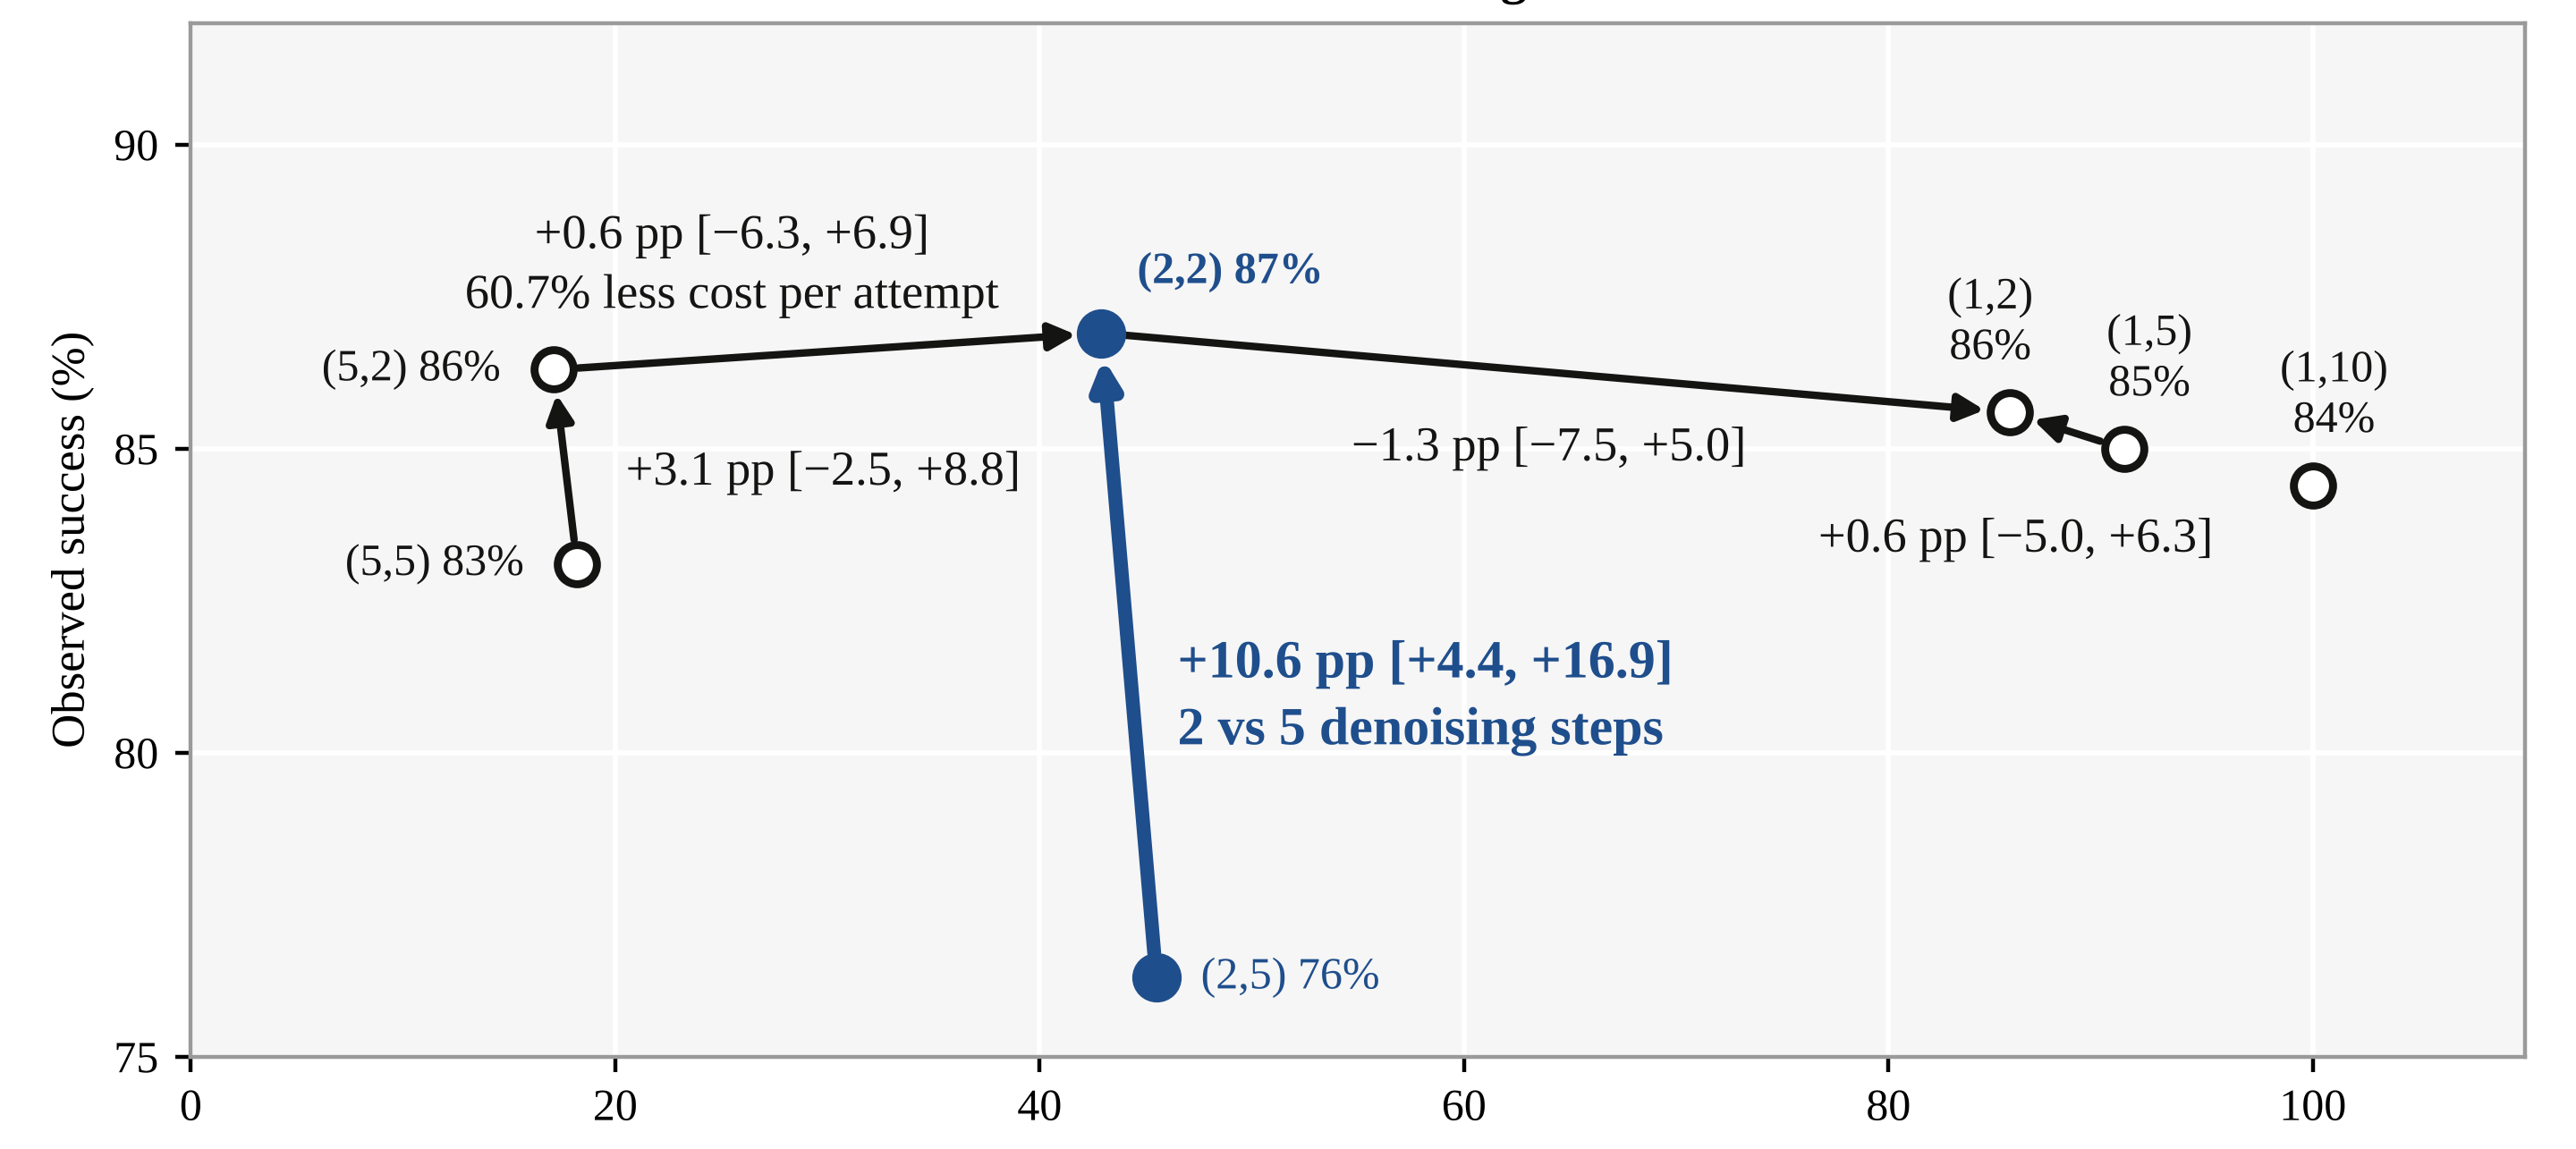
\includegraphics[width=\linewidth]{../paper/figures/fig_refinement_refresh_plot.png}\par\vspace{-0.4em}
{\small Compute per control step (\% of baseline)\par
$d=10,h=1$ is 100\%; lower values use less compute.}
\caption{SmolVLA case-study held-out success, compute, and paired comparisons.
Each point is one of the seven confirmation settings, labelled $(h,d)$ for
executed prefix and denoising count, and aggregates 160 attempts over eight tasks.
The vertical axis gives observed success and begins at 75\%. The horizontal axis
gives nominal counted generation arithmetic per control step as a percentage of
the native $(d=10,h=1)$ deployment baseline; leftward means less counted work per
executed action. Arrows run from comparator B to setting A and print the A-minus-B
success difference with its task-conditional, descriptive 95\% paired
state-bootstrap interval. Blue identifies the prespecified $(2,2)$ versus $(2,5)$
refinement test. Black arrows show two other frozen refinement comparisons and two
later-amended descriptive contrasts. The 60.7\% annotation is the separate
reduction in mean arithmetic per attempted episode for $(5,2)$ relative to
$(2,2)$; the associated $+0.6$-point success contrast does not establish
equivalent quality. The two additional amended contrasts involving $(1,10)$,
complete task-level outcomes, and full episode expenditures are reported in
Appendix~\ref{app:confirmation-details} and Table~\ref{tab:confirmation-grid}.}
\label{fig:success-compute}
\end{figure}
\FloatBarrier

\begin{table}[htbp]
\centering\small
\caption{Evidence status and permitted interpretation. Effects use A minus B.
The table separates prespecified confirmation from amended descriptive analysis.}
\label{tab:evidence-status}
\begin{tabular}{@{}p{0.18\linewidth}p{0.15\linewidth}p{0.26\linewidth}p{0.29\linewidth}@{}}
\toprule
Comparison & Status & Result & Supported claim\\
\midrule
$(2,2)-(2,5)$ & Frozen primary & $+10.6$ pp; 95\% interval $[+4.4,+16.9]$ &
At $h=2$, fewer denoising steps improved observed success for this checkpoint.\\
\addlinespace[2pt]
Other fixed-$h$ refinement tests & Frozen & Positive point estimates;
intervals span zero & A uniform benefit is not established for this checkpoint.\\
\addlinespace[2pt]
$(2,2)-(5,2)$ & \shortstack[l]{Amended\\descriptive} & $+0.6$ pp; 95\% interval $[-6.3,+6.9]$;
$(5,2)$ uses 60.7\% less arithmetic per attempt & The case study shows large
cost savings; equivalent quality is unresolved.\\
\bottomrule
\end{tabular}
\end{table}

\begin{samepage}
\subsection{Refinement: the frozen denoising comparisons}

For the case-study checkpoint, the primary two-action prefix with two denoising
steps yields 139/160 successes versus 122/160 for five steps. The paired difference is $+10.6$ percentage
points, with descriptive 95\% interval $[+4.4,+16.9]$, conditional on the eight
tasks. The selected setting also uses 5.9\% less nominal reference arithmetic
per control step: 275.0 versus 292.2 GFLOPs. Thus, in this SmolVLA comparison,
reducing refinement improves observed success while reducing counted work at
this fixed prefix.
\par\end{samepage}

Mean reference arithmetic per attempt falls from 48.7 to 41.1 TFLOPs
(15.6\%). This larger reduction includes changed trajectories and termination:
mean episode length is 149.0 versus 166.3 control steps. All failures reach
the task horizon (21 versus 38); the remaining attempts terminate successfully.
The primary direction is positive on seven tasks and tied on one, with
24 paired wins and seven losses. Appendix~\ref{app:primary-costs} gives
task sensitivity and expenditure intervals. These measurements do not establish
a controlled physical-latency improvement.
Figure~\ref{fig:success-compute} places the primary setting in the joint
success--compute coordinate and places its interval alongside all seven
confirmation contrasts.

Within the same checkpoint, the other two frozen tests have positive point estimates but intervals spanning
zero (Figure~\ref{fig:success-compute}). At $h=5$, two versus five
denoising steps give 138/160 versus 133/160 successes; at $h=1$, they give
137/160 versus 136/160. The largest observed benefit is at the primary prefix.
The primary gap exceeds its frozen prediction, while matching the signs of
three point estimates does not establish calibrated effect-size prediction.
These results do not demonstrate a uniform denoising benefit across prefixes.

\FloatBarrier
\subsection{Refresh: descriptive prefix comparisons}

Within the SmolVLA case study, we now hold denoising fixed and compare
expenditures on different refresh schedules. Table~\ref{tab:evidence-status} records the later amendment and the
claim boundary; Appendix~\ref{app:confirmation-details} gives full provenance.

At $d=2$, $(2,2)$ exceeds $(5,2)$ by just one success: 139/160 versus 138/160,
a paired difference of $+0.6$ percentage points $[-6.3,+6.9]$. Yet $(5,2)$ uses
60\% less nominal arithmetic per control step and 60.7\% less reference
arithmetic per attempt: 16.1 versus 41.1 TFLOPs. The interval permits meaningful
differences in either direction.
At task level, the $(5,2)-(2,2)$ difference is positive on three tasks,
negative on three, and tied on two (Table~\ref{tab:confirmation-tasks}). Thus
the near-equal aggregate counts contain mixed descriptive task-level changes.

Refreshing every action with $(1,2)$ instead of every two actions gives two
fewer successes, a difference of $-1.3$ points $[-7.5,+5.0]$, at 83.3 versus
41.1 TFLOPs per attempt. More frequent refresh has no demonstrated quality
benefit in these SmolVLA contrasts. Native-relative comparisons, which also change
denoising, are reported separately in Appendix~\ref{app:confirmation-details}.

Within the case study, the discovery point estimates favor shorter prefixes at $d=2$
(Section~\ref{sec:discovery-quality}), but their quality advantage is not
established on transfer. The task populations differ, so this comparison
does not identify a causal task effect. The cost model explains feasibility,
but does not determine the quality ranking on new tasks.

\section{Discussion and Conclusion}

This study develops a procedure for evaluating how chunked robot policies
allocate inference compute between refining an action prediction and refreshing
it from a new observation. The procedure measures the complete cost of a policy
call, separates configuration discovery from held-out confirmation, freezes the
confirmatory comparisons before evaluation, labels later contrasts as
descriptive, and reports closed-loop success together with episode expenditure.
This prevents a cheap configuration from being treated as useful without
behavioral evidence, or a successful configuration from being discussed without
its compute cost.

The transferable contribution is this evaluation protocol. SmolVLA serves as a
worked case study for one checkpoint and simulator stack, demonstrating how to
apply the procedure and how evidence status changes the permitted claims.
In this SmolVLA case study, additional refinement did not consistently produce
better closed-loop behavior. For this implementation, reducing refinement alone
delivered limited savings because most generation work was independent of
denoising. For this implementation, changing the execution prefix affected cost
more strongly, but similar observed success was insufficient to establish
equivalent quality. In the case study, the fitted response model also did not
improve configuration choices over a simple cost-aware rule. Refinement and refresh should therefore
be evaluated together within each model, under explicit counting boundaries,
with frozen confirmatory tests visibly separated from amended descriptive
analyses. These outcomes remain checkpoint-specific; broader allocation claims
require the same within-model study across other checkpoints, policy
architectures, tasks, and execution stacks.

\paragraph{Interpretation and limits.}
The two deployment controls are not isolated causal interventions on prediction
quality and observation freshness. Changing denoising changes numerical
integration; changing prefix changes both observation age and executed action
positions. The mechanism behind the observed primary difference remains open.
The study covers one checkpoint and twelve fixed tasks in simulation, with
only four discovery task-level validation folds. Intervals are task-conditional,
secondary contrasts are unadjusted, and no quality-preservation margin was
prespecified. The refresh-prefix contrasts were added after individual outcomes
were visible and remain descriptive. Two steps is the minimum denoising tested;
$d=1$ is untested.
The arithmetic boundary excludes several operation classes; language lengths
are audited but image shape is fixed. Sampled GPU checks have coverage gaps,
and simulated control steps do not establish real-time responsiveness.

\paragraph{Next steps.}
A matched stale-input diagnostic on the 40 discovery identities changes the
supplied images and proprioception refresh from every tick to every five ticks
while generating at every tick at $(h,d)=(1,5)$. Success falls from 28/40 with
fresh inputs to 20/40 with held inputs, a paired difference of $-20.0$ percentage
points with a descriptive task-conditional 95\% interval $[-32.5,-7.5]$.
This supports an observation-freshness contribution, but the step journal logs
action age rather than per-step supplied-input hashes or observation age; the
intervention therefore does not isolate every implementation detail. Completing
the input instrumentation and checking action positions can further separate
the mechanisms behind prefix effects.
A new, predeclared quality-preservation test for the cheaper $(5,2)$ setting
and replication on another policy are needed to assess whether its observed
cost advantage supports deployment. More broadly, the same study design can be
applied within other policies and simulator or robot stacks: define the refinement
and refresh controls, calibrate their complete inference cost, freeze the
confirmatory comparisons, and evaluate success and expenditure jointly. This
supports the broader objective of determining when the fixed cost of a fresh prediction is
worth paying and how much refinement that prediction needs.

\clearpage
\bibliographystyle{unsrtnat}
{\raggedright\bibliography{references}}
\clearpage
\appendix

\section{Detailed Outcomes and Resource Measurements}
\label{app:calibration}

{\raggedright
The checkpoint is \texttt{HuggingFaceVLA/smolvla\_libero}, revision
\texttt{6721902bc4d61e50a3bfdb11dfb4cb626f05d102}. Predicted chunk size is 50;
native execution uses $h=1,d=10$. Discovery uses Spatial tasks 5--8, initial
states 10--14, and policy seeds 2000 and 2001. The 20 task--state blocks
contain both seeds and all 12 configurations. Confirmation uses Goal and Object
tasks 5--8, states 20--29, and policy seeds 3000 and 3001. Its 80 task--state
blocks each contain both seeds and all seven configurations. Discovery bootstrap
resampling uses 20,000 draws with analysis seed 20260913.\par}

\begin{table}[htbp]
\centering\small
\caption{Discovery successes on Spatial tasks 5--8. Each task contributes five
states and two seeds per configuration. Rate/native is
$F_{\mathrm{gen}}(d)/(hF_{\mathrm{gen}}(10))$, not realized episode cost.
The best observed count is 28/40 at $(1,5)$; no monotonic denoising trend is
assumed.}
\label{tab:discovery-grid}
% Generated by render_paper_visuals.py; edit the renderer, not this file.
\begin{tabular}{@{}ccrrrrrS[table-format=1.3]@{}}
\toprule
\multicolumn{2}{c}{Allocation} & \multicolumn{4}{c}{Spatial task successes (each /10)} & & {Nominal}\\
\cmidrule(lr){1-2}\cmidrule(lr){3-6}
$h$ & $d$ & Task 5 & Task 6 & Task 7 & Task 8 & Total & {rate ratio}\\
\midrule
1 & 2 & 5 & 7 & 4 & 10 & 26/40 & 0.857\\
1 & 5 & 5 & 8 & 6 & 9 & 28/40 & 0.911\\
1 & 10 & 5 & 7 & 6 & 7 & 25/40 & 1.000\\
1 & 20 & 5 & 6 & 6 & 8 & 25/40 & 1.179\\
\addlinespace[3pt]
2 & 2 & 5 & 7 & 4 & 10 & 26/40 & 0.429\\
2 & 5 & 4 & 6 & 4 & 9 & 23/40 & 0.455\\
2 & 10 & 4 & 6 & 4 & 9 & 23/40 & 0.500\\
2 & 20 & 4 & 7 & 4 & 9 & 24/40 & 0.589\\
\addlinespace[3pt]
5 & 2 & 6 & 5 & 4 & 6 & 21/40 & 0.171\\
5 & 5 & 2 & 5 & 5 & 6 & 18/40 & 0.182\\
5 & 10 & 2 & 4 & 5 & 5 & 16/40 & 0.200\\
5 & 20 & 2 & 3 & 4 & 5 & 14/40 & 0.236\\
\bottomrule
\end{tabular}

\end{table}

\begin{figure}[htbp]
\centering
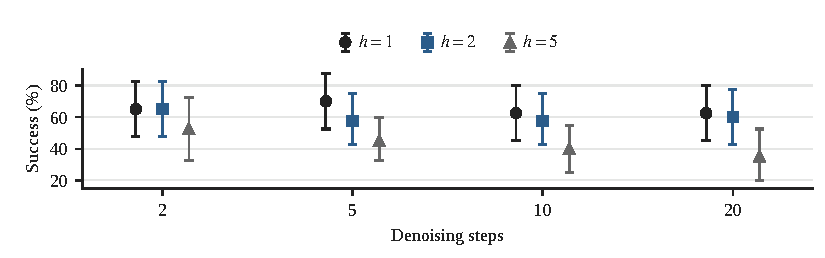
\includegraphics[width=\linewidth]{../paper/generated/discovery_success.pdf}
\caption{Discovery success by executed prefix $h$, with 40 attempts per
configuration on four Spatial tasks. Connected estimates make the within-prefix
response to denoising visible; whiskers are descriptive, task-conditional 95\%
paired state-bootstrap intervals. The $d$ axes are categorical.}
\label{fig:frontier}
\end{figure}

Calibration uses one real observation from Spatial task 0, initial state 0,
and common explicit noise. For each $d\in\{2,3,5,8,10,20\}$, profiling records
solver timesteps and dense operation counts, separately from elapsed timing.
Each setting receives 20 warm-up generations, followed by three randomized
timing blocks of 20 measured calls per setting. The rollout evaluator also
performs 20 warm-up generations once per configuration.

Host generation timing brackets prediction and completion synchronization;
CUDA events measure the current-stream prediction interval. The outer rollout
clock additionally includes observation processing, action handling,
simulation/rendering, and journal writes. Model loading, environment creation,
reset, and warm-up are measured separately. Process sampling occurs approximately
every five seconds; the largest recorded gap during discovery is below
5.03 seconds. Display processes remain on the measurement GPU.

\begin{table}[htbp]
\centering\small
\caption{Discovery resource measurements. Generated-chunk totals use the declared
dense-arithmetic boundary and charge partially executed final prefixes.
Episode means include unsuccessful attempts. $(2,2)$ has 26/40 observed
successes at 42.9\% of native arithmetic rate.}
\label{tab:resources}
% Generated by render_paper_visuals.py; edit the renderer, not this file.
\begin{tabular}{@{}ccS[table-format=3.1]S[table-format=3.1]S[table-format=3.1]r@{}}
\toprule
\multicolumn{2}{c}{Allocation} & {Nominal / step} & \multicolumn{2}{c}{Mean per attempt} & Success\\
\cmidrule(lr){1-2}\cmidrule(lr){3-3}\cmidrule(lr){4-5}
$h$ & $d$ & {GFLOPs} & {TFLOPs} & {Rollout (s)} & Count\\
\midrule
1 & 2 & 550.0 & 90.6 & 39.5 & 26/40\\
1 & 5 & 584.4 & 91.7 & 61.8 & 28/40\\
1 & 10 & 641.7 & 109.6 & 111.9 & 25/40\\
1 & 20 & 756.2 & 129.1 & 199.8 & 25/40\\
\addlinespace[3pt]
2 & 2 & 275.0 & 45.0 & 21.8 & 26/40\\
2 & 5 & 292.2 & 53.4 & 38.5 & 23/40\\
2 & 10 & 320.8 & 57.8 & 61.6 & 23/40\\
2 & 20 & 378.1 & 67.8 & 107.8 & 24/40\\
\addlinespace[3pt]
5 & 2 & 110.0 & 20.5 & 12.7 & 21/40\\
5 & 5 & 116.9 & 23.8 & 20.2 & 18/40\\
5 & 10 & 128.3 & 27.2 & 32.0 & 16/40\\
5 & 20 & 151.2 & 33.1 & 55.6 & 14/40\\
\bottomrule
\end{tabular}

\end{table}

Calibration requires approximately 291 seconds and discovery 31,245 seconds
(8.68 hours) of host elapsed time, including setup and bookkeeping. This search
expenditure is additional to subsequent deployments. The experiment does not
estimate an amortization threshold or a training--deployment cost crossover.

All measurements use an RTX 4060 Ti. Five-second process samples show no
unrelated CUDA compute process during calibration, discovery, or the initially
scheduled transfer phase; display processes remain. Process samples were not
retained for priority completion or the beginning of continuation. Later
continuation monitoring also shows no unrelated sampled CUDA compute process,
but these coverage gaps make aggregate transfer rollout times descriptive.
Host and CUDA-stream generation intervals are measured separately
from the outer synchronous rollout interval. Warm-up is excluded from these
rollout measurements.

\subsection{Fixed-input generation timing}
\label{app:fixed-timing}

\begin{table}[htbp]
\centering\small
\caption{Fixed-input full-generation calibration. Each setting has 60 calls in
three randomized blocks. Range gives the minimum and maximum host block means,
not a confidence interval. Host time falls more steeply with $d$ than counted
arithmetic. Host and CUDA columns average separate retained measurements of all
60 calls; the extra decimals distinguish their means, not timing accuracy.}
\begin{tabular}{@{}cS[table-format=3.1]S[table-format=4.3]S[table-format=4.3]r@{}}
\toprule
$d$ & {GFLOPs} & {Host (ms)} & {CUDA (ms)} & Host block range (ms)\\
\midrule
2 & 550.0 & 217.891 & 217.862 & 214.5--220.1\\
3 & 561.5 & 269.990 & 269.970 & 265.3--272.6\\
5 & 584.4 & 374.321 & 374.300 & 366.8--378.1\\
8 & 618.8 & 529.746 & 529.726 & 519.9--536.1\\
10 & 641.7 & 629.624 & 629.604 & 623.2--642.2\\
20 & 756.2 & 1158.635 & 1158.608 & 1133.5--1172.6\\
\bottomrule
\end{tabular}
\end{table}

The calibration stores full-generation intervals and global operator arithmetic
counts, not separate vision, language-prefill, or action-expert timings and
arithmetic totals. These records cannot attribute elapsed sensitivity to a
particular component, memory traffic, omitted operation classes, synchronization,
or software overhead. CUDA-event intervals are elapsed stream measurements,
not summed active-kernel durations. No component-level decomposition is inferred.

\subsection{Resource-coordinate sensitivity}
\label{app:timing-sensitivity}

Arithmetic savings and elapsed savings differ. Mean rollout time is 111.9 seconds
per attempt for native deployment, 61.8 seconds for $(1,5)$, and 21.8 seconds for
$(2,2)$. Their mean generated-chunk expenditures are 109.6, 91.7, and 45.0 TFLOPs,
respectively. These are observed all-attempt means under the same task allocation;
they include different trajectories and outcomes. Table~\ref{tab:resources}
reports all discovery configurations.

There is also an ordering reversal: $(1,5)$ uses more arithmetic per attempt
than $(2,20)$ (91.7 versus 67.8 TFLOPs), but less rollout time (61.8 versus
107.8 seconds). These means include different trajectories. On a fixed input,
reducing $d$ from 10 to 5 lowers mean generation host time from 629.6 to
374.3 ms (40.5\%), despite only 8.9\% less counted arithmetic. The calibration
therefore also separates arithmetic savings from elapsed savings without
trajectory differences. It does not resolve their component-level cause.
A FLOP-constrained choice is not necessarily a latency- or throughput-optimal
choice.

As a descriptive sensitivity analysis, define calibrated host-time rate
$b_T(h,d)=\overline{T}_{\mathrm{gen}}(d)/h$, the amortized fixed-input generation
time per simulated control step, and normalize it by native host-time rate.
For $(1,2)$, $(2,2)$, and $(5,2)$, the normalized arithmetic rates are
0.857, 0.429, and 0.171, while the normalized host-time rates are 0.346, 0.173,
and 0.069. Consequently, $(1,2)$ is ineligible at a half-native arithmetic
ceiling but eligible at a separately normalized half-native host-time ceiling.
These resource constraints admit different refresh schedules; the choices do
not establish quality optima. The frozen experiment remains arithmetic-based.

\subsection{Language-shape transport audit}
\label{app:shape-audit}

The profiled batch contains one sample, two $3\times360\times360$ image tensors,
an eight-dimensional state tensor, and language-token and attention-mask tensors
of length 20. The checkpoint exposes seven-dimensional actions and generates a
50-action chunk. Evaluation fixes batch size, image preprocessing, state/action
dimensions, and chunk size. The tokenizer pads language only to the longest
sequence in a batch. Reconstructing the declared task strings with the pinned
tokenizer gives 15--17 tokens for discovery and 5--12 for transfer, versus 20
in calibration. We profile every distinct evaluated length for
$d\in\{2,5,10\}$, preserving all other shapes, and test eligibility against
the original absolute ceilings. Table~\ref{tab:shape-audit} reports the range
over evaluated lengths 5--17 against the original length-20 value.

\begin{table}[htbp]
\centering\small
\caption{Dense generation arithmetic across evaluated language shapes. Budget
tests retain the original absolute ceilings; none of the reported transfer
configurations changes eligibility.}
\label{tab:shape-audit}
\begin{tabular}{@{}crS[table-format=3.1]c@{}}
\toprule
$d$ & \shortstack{Evaluated lengths\\GFLOPs (range)} & {\shortstack{Length 20\\GFLOPs}} & \shortstack{Eligibility\\changes}\\
\midrule
2  & 539.7--547.9 & 550.0 & 0\\
5  & 573.5--582.2 & 584.4 & 0\\
10 & 629.8--639.3 & 641.7 & 0\\
\bottomrule
\end{tabular}
\end{table}

In particular, $(2,10)$ remains within the original half-native ceiling for all
evaluated lengths; shorter inputs reduce rather than increase its counted work.
The audit changes neither policy execution nor the frozen selections.

\subsection{Primary expenditure and runtime}
\label{app:primary-costs}

The primary selected configuration $(2,2)$ has a higher success count than
$(2,5)$ on seven tasks and ties on one (Table~\ref{tab:primary-tasks}).
There are 24 paired wins and seven
losses. In a descriptive leave-one-task-out sensitivity analysis, the
equally weighted difference over the remaining seven tasks stays positive,
ranging from 9.3 to 12.1 percentage points. This post-outcome analysis does not
extend inference to a new task population. The supplementary paired records
retain all state and seed identities needed to reproduce the primary interval.

\begin{table}[htbp]
\centering\small
\caption{Descriptive primary expenditure differences, selected minus comparator
at $h=2$, including all attempts. Intervals use the paired state bootstrap
conditional on the eight tasks and were added after outcomes were observed.
Timing intervals summarize sampling variation in the observed records; they
do not account for unmonitored runtime interference during priority completion.}
\label{tab:primary-costs}
% Generated by render_paper_visuals.py; edit the renderer, not this file.
\begin{tabular}{@{}lS[table-format=3.1]S[table-format=3.1]S[table-format=-2.1]l@{}}
\toprule
Mean per attempt & {$d=2$} & {$d=5$} & {Difference} & 95\% interval\\
\midrule
Reference TFLOPs & 41.1 & 48.7 & -7.6 & $[-10.6,\,-4.5]$\\
Observed rollout (s) & 19.0 & 34.3 & -15.2 & $[-17.2,\,-13.3]$\\
Control steps & 149.0 & 166.3 & -17.3 & $[-27.9,\,-6.5]$\\
\bottomrule
\end{tabular}

\end{table}

\begin{table}[htbp]
\centering\small
\caption{Runtime and protocol shared by all four confirmation execution phases.
Module versions are the loaded versions reported at evaluation time. The
supplement retains source digests and distinguishes conflicting installed
distribution metadata from these loaded versions.}
\label{tab:runtime}
\begin{tabular}{@{}>{\raggedright\arraybackslash}p{0.24\linewidth}>{\raggedright\arraybackslash}p{0.71\linewidth}@{}}
\toprule
Setting & Value\\
\midrule
Hardware & RTX 4060 Ti, 16 GB; driver 595.84\\
Runtime & Python~3.12.3; PyTorch~2.7.1+cu126; CUDA~12.6;\newline NumPy~2.2.6; MuJoCo~3.8.1\\
\addlinespace[3pt]
Evaluation & Batch 1; synchronous simulation; nominal 20 Hz (50 ms control period)\\
Episode horizons & Spatial and Object: 280 control steps; Goal: 300\\
\addlinespace[3pt]
Precision controls & Autocast and TF32 disabled; deterministic algorithms enabled\\
Attention and reuse & Eager language/action attention with float32 scores; within-generation KV cache enabled\\
Compilation/warm-up & Model compilation disabled; 20 warm-up generations per condition\\
\addlinespace[3pt]
Evaluator source & \texttt{run\_paired.py}; SHA-256 prefix\newline \texttt{516375133d030ff4} (full digest in supplement)\\
\bottomrule
\end{tabular}
\end{table}

The manifests do not retain a parameter-dtype inventory or a separate vision
attention-backend inventory. The attention details in Table~\ref{tab:runtime} follow the pinned
language/action implementation; they do not identify every runtime kernel.

\subsection{Complete confirmation outcomes}
\label{app:confirmation-details}

\begin{table}[htbp]
\centering\small
\caption{Confirmation successes by task and configuration. Each task row has
20 attempts: ten paired initial states, each with two policy seeds. The total
aggregates 160 attempts per configuration. The primary
$(2,2)$ setting exceeds $(2,5)$ on seven tasks and ties on one.}
\label{tab:primary-tasks}
\label{tab:confirmation-tasks}
% Generated by render_paper_visuals.py; edit the renderer, not this file.
\begin{tabular}{@{}lS[table-format=3.0]S[table-format=3.0]S[table-format=3.0]S[table-format=3.0]S[table-format=3.0]S[table-format=3.0]S[table-format=3.0]@{}}
\toprule
 & \multicolumn{3}{c}{$h=1$} & \multicolumn{2}{c}{$h=2$ (primary pair)} & \multicolumn{2}{c}{$h=5$}\\
\cmidrule(lr){2-4}\cmidrule(lr){5-6}\cmidrule(l){7-8}
Task & {$d=2$} & {$d=5$} & {$d=10$} & {$d=2$} & {$d=5$} & {$d=2$} & {$d=5$}\\
\midrule
Goal 5 & 14 & 15 & 14 & 16 & 14 & 18 & 16\\
Goal 6 & 18 & 17 & 17 & 18 & 15 & 19 & 18\\
Goal 7 & 20 & 20 & 20 & 19 & 18 & 18 & 18\\
Goal 8 & 19 & 18 & 18 & 18 & 14 & 18 & 15\\
\addlinespace[3pt]
Object 5 & 20 & 19 & 19 & 20 & 20 & 20 & 20\\
Object 6 & 19 & 18 & 19 & 20 & 17 & 18 & 18\\
Object 7 & 9 & 9 & 10 & 10 & 7 & 7 & 8\\
Object 8 & 18 & 20 & 18 & 18 & 17 & 20 & 20\\
\midrule
Total (/160) & 137 & 136 & 135 & 139 & 122 & 138 & 133\\
\bottomrule
\end{tabular}

\end{table}

\begin{table}[htbp]
\centering\small
\caption{Amended descriptive comparisons using all 160 attempts per setting.
These contrasts were documented after collection began and are not originally
prespecified or fully outcome-blind. Intervals are task-conditional,
unadjusted, and do not test a quality-preservation margin.}
\label{tab:confirmation-secondary}
% Generated by render_paper_visuals.py; edit the renderer, not this file.
\begin{tabular}{@{}ccS[table-format=+2.1]l@{}}
\toprule
Setting A & Setting B & {A$-$B (pp)} & 95\% interval (pp)\\
\midrule
$(2,2)$ & $(1,10)$ & +2.5 & $[-3.8,\,+8.1]$\\
$(2,2)$ & $(5,2)$ & +0.6 & $[-6.3,\,+6.9]$\\
$(1,2)$ & $(2,2)$ & -1.3 & $[-7.5,\,+5.0]$\\
$(1,2)$ & $(1,10)$ & +1.3 & $[-5.0,\,+7.5]$\\
\bottomrule
\end{tabular}

\end{table}

The stale-input intervention is reported separately from the confirmation
comparisons. It is a 40-attempt mechanism diagnostic on the discovery identities,
not an additional confirmation configuration. The held-input and matched
fresh-input records share all 40 initial state and observation hashes; the stale
run's remote artifacts are retained with their own manifest and schedule hashes.

The four amended comparisons are reported in their documented order, using
20,000 paired state-bootstrap resamples and analysis seed 20260913.
Table~\ref{tab:confirmation-grid} gives their all-attempt resource means.
In particular, the $(2,2)$ minus $(5,2)$ expenditure difference is
$+25.0$ TFLOPs per attempt, with descriptive interval $[+22.8,+27.5]$.
This interval describes generated-chunk arithmetic, including the different
trajectory lengths; it is not an elapsed-time comparison or evidence of
equivalent quality.

\FloatBarrier
\paragraph{Measurement verification.}
\phantomsection
\label{app:verification}

The retained records support a complete internal reconciliation of planned
identities, paired states, executed actions, and recorded outcomes. The checks
below constrain recording and execution errors; they do not constitute an
independent outcome replay in a separate simulator.

\begin{table}[htbp]
\centering\small
\caption{Internal measurement-verification checklist.}
\label{tab:verification-summary}
\begin{tabular}{@{}p{0.25\linewidth}p{0.67\linewidth}@{}}
\toprule
Check & Evidence\\
\midrule
Canonical coverage & 1,120 confirmation attempts and 171,805 actions; the
primary subset remains 320 attempts and 50,451 actions.\\
Pairing and dispatch & Planned identities, paired initial states and
observations, generation counts, denoising counts, and applied actions reconcile.\\
Excluded records & Two repeated completed attempts are checked and excluded;
one interrupted ten-action record has no completed outcome and is excluded.\\
Outcome path & All 1,122 raw completed records and 172,243 steps reconcile;
generated actions match simulator actions and recorded outcome fields agree.\\
Shared predicate & Reward and success both use LIBERO's task-goal evaluation,
traced to BDDL predicates, so their agreement is an internal consistency check.\\
Native parity & One Spatial episode matches the upstream path in initial state,
observation, 70-action sequence, length, and outcome.\\
Remaining boundary & Independent, version-matched replay and direct terminal-state
inspection remain outside this audit.\\
\bottomrule
\end{tabular}
\end{table}
\FloatBarrier
\paragraph{Analysis provenance.}
\phantomsection
\label{app:analysis-provenance}

The three refinement comparisons, identities, and primary analysis were frozen
before transfer outcomes. A deadline-driven amendment changed only execution
order after 114 attempts per primary setting had been recorded; settings,
identities, stopping rules, and inclusion remained fixed. Continuation completed
the original identities, and deduplication retained the earliest completed
record under the documented phase precedence. The frozen analyses use seed
20260912. Amended prefix contrasts and diagnostics use seed 20260913 and are
descriptive because they were added after collection began. No response model
was refitted on confirmation outcomes.

\paragraph{Analysis artifact.}
The accompanying \texttt{primary\_transfer\_supplement.zip} contains the primary
episode and action records, original planned identities, paired state values,
calibrations, frozen predictions, runtime extract, and analysis code.
Running \texttt{python primary\_reporting.py --check .} reproduces the primary
counts, interval, task table, and descriptive expenditure analysis without
inference. Its README specifies the selector features, penalized objective,
candidate set, and normalization. Machine-specific paths are omitted from the
runtime extract; checkpoint weights and simulator assets are not bundled.
The continuing repository additionally retains a compressed completed-confirmation
snapshot and \texttt{analyze\_confirmation.py}. Its \texttt{--check} mode
reconciles the full journals, original schedule, runtime manifests, repeated
identities, and paired blocks, then reproduces the seven-setting resource table,
all original and amended comparisons, and task-level counts. Generated evidence
records source, input, and snapshot hashes. The submitted supplement remains
separate from these post-submission additions.

\FloatBarrier
\section{Frozen Selection and Diagnostic Analyses}
\label{app:selectors}

We compare two logistic response-model families. A compute-only model uses a
quadratic in log normalized rate. An allocation model uses $\log h$,
$\log(d/10)$, both squared terms, and their interaction. Each family is fitted
with ridge penalty 1 or 10. Leave-one-task-out log loss selects the model, which
is then refitted on the discovery set. No individual seed repeat is held out
while another repeat from the same task remains in training.

The candidate set is $h\in\{1,2,3,5\}$ crossed with $d\in\{2,3,5,8,10,20\}$:
the 12 discovery configurations and 12 untested configurations. Their calibrated costs determine
eligibility; the fitted model selects the highest predicted success under each
ceiling. Ties favor lower compute, then lexicographic order.

\begin{table}[htbp]
\centering\small
\caption{Discovery-based selector choices.
The learned choices and comparisons were frozen before transfer; additional
selector baselines were documented after collection began.
The empirical selector uses the measured grid; other selectors use the declared
candidate set. The simple rule exactly matches the learned choices. Selected
rate/native is the learned recommendation's arithmetic rate. Frozen comparators
and predicted gaps appear in Table~\ref{tab:confirmation-predictions};
the half-native row is primary.
}
\label{tab:selectors}
\label{tab:predictions}
% Generated by render_paper_visuals.py; edit the renderer, not this file.
\begin{tabular}{@{}lccccS[table-format=1.3]@{}}
\toprule
 & \multicolumn{4}{c}{Selector choice $(h,d)$} & {Learned}\\
\cmidrule(lr){2-5}
Ceiling/native & Learned & Simple & Empirical & Compute-only & {rate/native}\\
\midrule
0.25 & $(5,2)$ & $(5,2)$ & $(5,2)$ & $(5,20)$ & 0.171\\
0.50\ (primary) & $(2,2)$ & $(2,2)$ & $(2,2)$ & $(2,10)$ & 0.429\\
1.00 & $(1,2)$ & $(1,2)$ & $(1,5)$ & $(1,10)$ & 0.857\\
\bottomrule
\end{tabular}

\end{table}

\begin{table}[htbp]
\centering\small
\caption{All original frozen denoising tests: selected minus comparator,
holding $h$ fixed within each row. Predicted and observed gaps and intervals are
percentage points. The half-native row is primary; secondary intervals are
descriptive, task-conditional, and unadjusted.}
\label{tab:confirmation-predictions}
% Generated by render_paper_visuals.py; edit the renderer, not this file.
\begin{tabular}{@{}lccS[table-format=+2.1]S[table-format=+2.1]l@{}}
\toprule
Ceiling & \multicolumn{2}{c}{Setting $(h,d)$} & \multicolumn{3}{c}{Success difference (pp)}\\
\cmidrule(lr){2-3}\cmidrule(l){4-6}
/ native & Selected & Comparator & {Predicted} & {Observed} & {95\% interval}\\
\midrule
0.25 & $(5,2)$ & $(5,5)$ & +6.5 & +3.1 & $[-2.5,\,+8.8]$\\
0.50\ (primary) & $(2,2)$ & $(2,5)$ & +4.0 & +10.6 & $[+4.4,\,+16.9]$\\
1.00 & $(1,2)$ & $(1,5)$ & +2.2 & +0.6 & $[-5.0,\,+6.3]$\\
\bottomrule
\end{tabular}

\end{table}

The simple rule minimizes denoising count, then chooses the shortest feasible
prefix. It reproduces every learned recommendation (Table~\ref{tab:selectors});
transfer outcomes cannot distinguish these selectors at the tested budgets.
The compute-only choices use the original ridge-10 fit. Its quarter- and
half-budget choices are absent from the transfer plan, so this evaluation
cannot compare those decisions on transfer tasks.

The selected allocation model has log loss 0.7048, compared with 0.7067 for the
best compute-only model. This small difference provides no evidence of an added
predictive advantage. Under the same mean natural-log binary cross-entropy,
constant $p=0.5$ scores 0.6931 and an intercept-only model fitted separately on
each training fold scores 0.7170. The response-model probabilities should
therefore not be read as calibrated task-transfer forecasts. The primary test
evaluates a recommendation shared with simpler selectors, so it does not
establish an additional benefit from model-based ranking.

\end{document}
